\documentclass[a4paper]{ctexart}
\usepackage{xeCJK}

\setCJKmainfont[BoldFont={方正大黑简体}, ItalicFont={方正盛世楷书简体_准}, BoldItalicFont={方正大标宋简体}]{方正标雅宋简体}
\setCJKsansfont{方正兰亭细黑简体}
\setCJKmonofont{仿宋}

\title{配重式全向球形机器人}
\author{马力全关组}

% Math
\usepackage{amsthm, amsmath, amssymb}
\usepackage{mathrsfs}
% Utility
\usepackage{graphicx}
\usepackage{subfigure}
\usepackage{lastpage}
% Beautifying packages
\usepackage{wallpaper}
% Code related
\usepackage{minted, framed}
\usepackage{listings}
\usepackage[linesnumbered,boxed]{algorithm2e}
% Formatting
\usepackage{footmisc}
\usepackage{float}
\usepackage{longtable, array, booktabs}
\usepackage{fancyhdr}
\usepackage{tcolorbox, framed}
\usepackage{geometry}
\usepackage{multicol}
%\usepackage[toc]{multitoc}
\usepackage{hyperref}
% tikz
\usepackage{xcolor}
\usepackage{tikz}
\usetikzlibrary{arrows,shapes,chains}


\tikzstyle{startstop}=[rectangle,rounded corners,minimum width=3cm,minimum height=1cm,text centered,draw=black,fill=red!30]
\tikzstyle{process}=[rectangle,minimum width=3cm,minimum height=1cm,text centered,text width =3cm,draw=black,fill=orange!30]
\tikzstyle{arrow}=[thick,->,>=stealth]

% Macro definitions
\usepackage{color}
\definecolor{grey}{RGB}{190, 190, 190}
\geometry{a4paper,left=2.8cm,right=2.8cm,top=3.2cm,bottom=3.2cm}
\newcommand{ \upcite}[1]{\textsuperscript{\textsuperscript{\cite{#1} } }}
\newcommand{ \mathbit}[1]{\mathbf{\mathit{#1}}}
\hypersetup{
colorlinks=true,
linkcolor=black
}
\numberwithin{equation}{section}
\numberwithin{table}{section}
\numberwithin{figure}{section}

\setlength{\columnseprule}{0.8pt}
\setlength\columnsep{1cm}


%%%%%%%%%%%%%%%%%%

\begin{document}
\setboolean{@twoside}{true}


\begin{titlepage}

  \maketitle
  \begin{center}
    小组课程实践
  \end{center}

  \ThisLRCornerWallPaper{0.8}{cover.png}

  \begin{longtable}[]{@{}ccc@{}}
  \toprule
  成员 & 姓名 & 联系电话\tabularnewline
  \midrule
  \endhead
  组长 & 张骏扬 & 18967993817\tabularnewline
  执行组长 & 曲凌枫 & \tabularnewline
  机械组 & 马博楠 & \tabularnewline
  电子组 & 栾家骏 & \tabularnewline
  软件组 & 戴嘉琦 & \tabularnewline
  \bottomrule
  \end{longtable}
  \addtocounter{table}{-1}

  
\begin{center}
  创新思维和机器人创客实践
\end{center}

\thispagestyle{empty}

\end{titlepage}

\addtocounter{page}{-2}

\newpage

\thispagestyle{fancy}
\lhead{}
\chead{\it\small{\textcolor{grey}{目录}}}
\rhead{}
\cfoot{}

\tableofcontents

\newpage


% now body
\pagestyle{fancy}
\fancyhead[RE, LO]{\it\small\rightmark}
\fancyhead[C]{\small{\it\textcolor{grey}{配重式球形机器人}}}
\fancyhead[LE, RO]{\it\small{马力全关组}}
\fancyfoot[C]{\it\small{第 \thepage 页\ 共 \pageref{LastPage} 页}}

\section{问题提出}

\subsection{设计背景与目的}

本组所建立的配重式全向球形机器人项目是西安交通大学课程“创新思维和机器人创客实践”的机器人小组实践项目。设计目的是:

\begin{itemize}
  \item 进行团队组织实践,使用团队组织技巧,锻炼合作能力;
  \item 进行产品调研与开发实践,锻炼创新能力;
  \item 进行机械、电子、软件设计实践,锻炼学习与设计能力
  \item 进行系统统调装配,锻炼排错与优化能力。
\end{itemize}

\subsection{国内外现有研究成果}

配重式全向球形机器人最初的设计概念在 2004 年被提出\upcite{2004Introducing}。

\section{需求分析}

\subsection{需求分析和筛选}

球形形态机器人可衡量的目标有以下几点:

\begin{itemize}
  \item 全向对称移动:在球形机器人的任何状态能够以任意方向继续滚动,使得在地面斜率变化的情况下可以使用算法保持稳定的运动路线;
  \item 精密控制能力:配重式球形机器人能够进行精密的
  \item 通过性:同尺寸球形机器人相较其他形态拥有较强的通过性,适应不平整地形;
  \item 机械强度与密闭性:球形机器人可以使用无线控制方式,使得球壳能够完全密闭,防水抗干扰;
\end{itemize}

\subsection{关键痛点的提炼}

\section{设计概念生成、选择、评估与实现}


\subsection{概念的生成}

下面介绍本项目按时间阶段拟设计的四种机器人方案。

\subsubsection{设计概念一——六足式机器人}

最初,本项目拟设计制作六电机六足式机器人,并使用该设想进行初步立项。该设想被否决,原因是已有成熟的商业产品先例以及开源项目,无法体现创新性。


\subsubsection{设计概念二——三足式弹跳机器人}

六足机器人否决后,本项目拟设计制作小型化三足式弹跳机器人。


\subsubsection{设计概念三——重心牵拉式球形机器人}

由于三足式机器人的流产,本项目将方向转变为球形机器人。

\subsubsection{设计概念四——配重式球型机器人}



\subsection{概念选择与评估}


\section{概念的具体设计}

\subsection{机械系统设计}

\begin{figure}[H]
  \begin{minipage}{0.32\linewidth}
    \begin{center}
      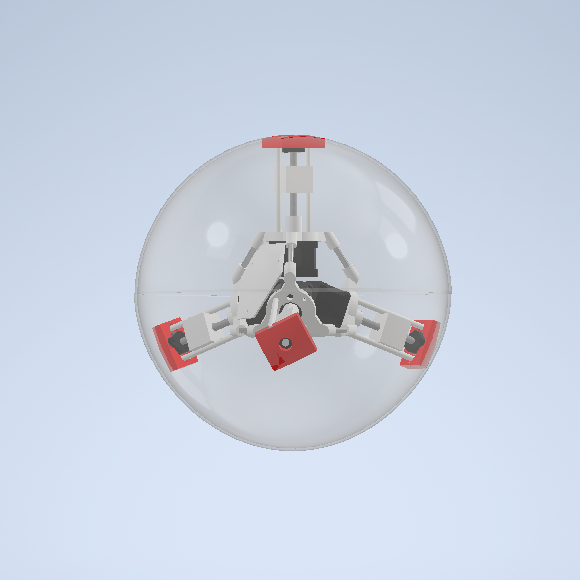
\includegraphics[width=0.98\linewidth]{figures/rendered1.png}
    \end{center}
  \end{minipage}
  \hfill
  \begin{minipage}{0.32\linewidth}
    \begin{center}
      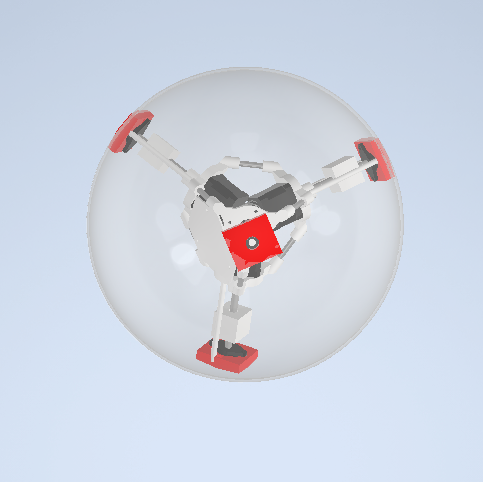
\includegraphics[width=0.98\linewidth]{figures/rendered2.png}
    \end{center}
  \end{minipage}
  \hfill
  \begin{minipage}{0.32\linewidth}
    \begin{center}
      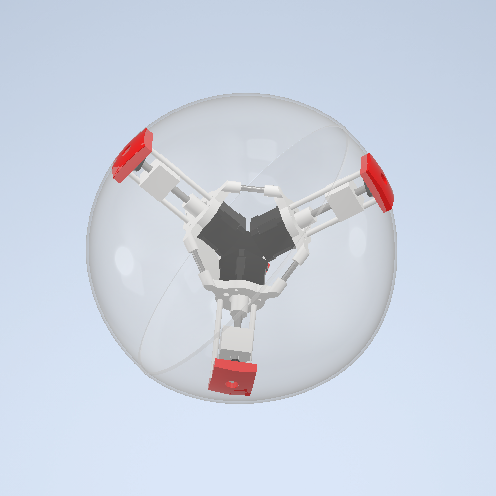
\includegraphics[width=0.98\linewidth]{figures/rendered3.png}
    \end{center}
  \end{minipage}
  \caption{机械结构 CAD 设计渲染图}
\end{figure}

\subsection{电子系统设计}

\subsection{控制算法设计}

经讨论,考虑到实现可行性,本项目采用位置反馈控制而不是文献中描述的 PID 速度控制。下面简要介绍我组实现(及拟实现)的控制算法原理。

\subsubsection{坐标系统}

球形机器人依赖两种坐标系统:相对坐标系与绝对坐标系。相对坐标系是指相对于球心,方向为球壳某定点的球坐标系;绝对坐标系是指相对于地面的坐标系。在无特殊说明的情况下采用相对坐标系统。

球坐标系中,点定义为 $(\rho, \theta, \phi)$,$\rho\ge 0$ 是距离球心的位置,$\theta \in [0,2\pi)$,$\phi \in [-\pi, \pi]$ 是极角,定义为经纬弧度坐标。

球坐标到平面直角坐标的转换如下:

\begin{equation}
\begin{cases}
  x = \rho\sin\phi\cos\theta \\
  y = \rho\sin\phi\sin\theta \\
  z = \cos\phi \\
\end{cases}
\end{equation}

在该相对坐标系内,四组配重运动方向向量在直角坐标系下分别定义为:

\begin{align}
  \boldsymbol v_0 & = (0,0,R_0) \\
  \boldsymbol v_1 & = (\dfrac{2\sqrt{2}}{3}R_0,0,\dfrac{1}{3}R_0) \\
  \boldsymbol v_2 & = (-\dfrac{\sqrt{2}}{3}R_0,\dfrac{\sqrt{6}}{3}R_0,-\dfrac{1}{3}R_0) \\
  \boldsymbol v_3 & = (-\dfrac{\sqrt{2}}{3}R_0,-\dfrac{\sqrt{6}}{3}R_0,-\dfrac{1}{3}R_0)
\end{align}

我们将机器人配重块所处位置的状态定义为移动至上限 $u\boldsymbol v_i$ 与下限 $l\boldsymbol v_i$ 之间的比例 $p_i\in[0,1]$,$i = 0,1,2,3$。设单个配重块质量为 $m$,机器人除配重块外的质量为 $M$,则有机器人重心位置 $\boldsymbol c$:

\begin{equation}
  \boldsymbol c = \frac{\sum_i m [l + (u-l) p_i] \boldsymbol v_i}{M + 4m} = \frac{m (u-l)}{M + 4m}\sum_i p_i \boldsymbol v_i \triangleq C \sum_i p_i \boldsymbol v_i
  \label{equ_center}
\end{equation}

其中常量 $C=\dfrac{m (u-l)}{M + 4m}$,以下规定 $\overline{\boldsymbol c} = \dfrac{\boldsymbol c}{C} = \sum_i p_i \boldsymbol v_i$

\subsubsection{位置求解}

当机器人在低速情况时,可假设中心与重心的射线始终指向地心,也就是说,只要改变机器人重心在相对坐标系中的位置,产生滚动,就可以改变机器人中心在绝对坐标系中的位置,并且位置是确定的。下文给出一种确定性连续求解位置的方法,目的是把机器人位移指令转换的重心位置串,继续转换为配重块位置串。

当给定中心位置 $\overline{\boldsymbol c}$,因式\ref{equ_center}是超定方程,拥有多解,不能立刻求出四个配重位移比例。则以电机对称调用、尽量靠近杆中心为目标,给出一个合理的求解方法。若忽略 $\boldsymbol v_3$,由于 $\boldsymbol v_0,\boldsymbol v_1,\boldsymbol v_2$ 正交,以此三个向量作为基向量,可解出 $\overline{\boldsymbol c}$ 的分解 $\left(p_0^{(3)},p_1^{(3)},p_2^{(3)}\right)$。又有 $\boldsymbol v_3 = - \boldsymbol v_0 -\boldsymbol v_1-\boldsymbol v_2$,则可以得到一个尽量靠近杆中心的非对称解:

\begin{equation}
  \left(p_0^{(3)} +\frac{1}{2}, p_1^{(3)} +\frac{1}{2}, p_2^{(3)} + \frac{1}{2}, \frac{1}{2}\right)
\end{equation}

同理,我们可以解出 $\left(p_0^{(2)},p_1^{(2)},p_3^{(2)}\right)$,$\left(p_0^{(1)},p_2^{(1)},p_3^{(1)}\right)$,$\left(p_1^{(0)},p_2^{(0)},p_3^{(0)}\right)$,将非对称解平均,即可得到一个对称解:

\begin{equation}
  \left(
    \frac{p_0^{(1)}+p_0^{(2)}+p_0^{(3)}}{4} +\frac{1}{2},
    \frac{p_1^{(0)}+p_1^{(2)}+p_1^{(3)}}{4} +\frac{1}{2},
    \frac{p_2^{(0)}+p_2^{(1)}+p_2^{(3)}}{4} +\frac{1}{2},
    \frac{p_3^{(0)}+p_3^{(1)}+p_3^{(2)}}{4} +\frac{1}{2}
  \right)
\end{equation}

由向量内积,有 $p_i^{(j)} = \overline{\boldsymbol c} \cdot \boldsymbol v_i$,也可通过线性方程组
\ref{equ_linear_solve}求解。

\begin{equation}
  \begin{bmatrix}
    \boldsymbol v_{i_0} \\
    \boldsymbol v_{i_1} \\
    \boldsymbol v_{i_2} \\
  \end{bmatrix}
  \begin{bmatrix}
    p_{i_0}^{(i_3)} \\
    p_{i_1}^{(i_3)} \\
    p_{i_2}^{(i_3)} \\
  \end{bmatrix}
  =
  \overline{\boldsymbol c}
  \label{equ_linear_solve}
\end{equation}

其中 $i_0\neq i_1\neq i_2\neq i_3$。


\subsubsection{运动方向与大地坐标}

由于相对坐标与绝对坐标不平行,在算法描述机器人状态时,除了相对坐标下的重心方向 $\overline{\boldsymbol c}$,还需要相对坐标下的前进方向 $\boldsymbol d$,其有两种实现方法,第一种是基于传感器获得绝对坐标;另一种是通过微分获得相对坐标的前进方向,定义为 $\boldsymbol d=\dfrac{\mathrm d\boldsymbol c}{\mathrm d t}$。本项目由于时间限制,暂时采用微分方式,其实现为有限差分。

当传入改变前进方向的指令时,首先由摇杆信息 $(a,b)$ 转换为平面极坐标 $\theta \in [-pi,pi)$,则需要使 $\boldsymbol d$ 沿轴 $\overline{\boldsymbol c}$ 旋转角度 $\theta$,设平面直角坐标下 $\boldsymbol d=(x,y,z)$,$\overline{\boldsymbol c}=(u,v,w)$,有旋转方程:

\begin{equation}
  \begin{bmatrix}
    x^{(n+1)} \\
    y^{(n+1)} \\
    z^{(n+1)} \\
    1
  \end{bmatrix}
  =
  \begin{bmatrix}
    u^2+(1-u^2)\cos\theta & uv(1-\cos\theta)-w\sin\theta & uw(1-\cos\theta)+v\sin\theta & 0\\
    uv(1-\cos\theta)+w\sin\theta & v^2+(1-v^2)\cos\theta & vw(1-\cos\theta)-u\sin\theta & 0\\
    uw(1-\cos\theta)-v\sin\theta & vw(1-\cos\theta)+u\sin\theta & w^2+(1-w^2)\cos\theta & 0\\
    0 & 0 & 0 & 1
  \end{bmatrix}
  \begin{bmatrix}
    x^{(n)} \\
    y^{(n)} \\
    z^{(n)} \\
    1
  \end{bmatrix}
\end{equation}

此时若有控制指令序列 $\{(a_i,b_i)\}$,即可得到位置序列 $\{\overline{\boldsymbol c}_i\}$ 与方向序列 $\{\boldsymbol d_i\}$,有 $\overline{\boldsymbol c}_i = \overline{\boldsymbol c}_{i-1} + v\boldsymbol d_i$,其中 $v$ 为输入速度。综上即可完成机器人的指令控制。

\section{概念原型化和实践总结}

\subsection{概念的原型化结果}



\subsection{创新实践总结}

\newpage
\thispagestyle{fancy}
\lhead{}
\chead{\it\small{\textcolor{grey}{参考文献}}}
\rhead{}
\fancyfoot[C]{\it\small{第 \thepage 页\ 共 \pageref{LastPage} 页}}
\phantomsection
\addcontentsline{toc}{section}{参考文献}
\bibliography{mycitation}
\bibliographystyle{gbt7714-2005}
%\printbibliography


\end{document}
